%!TEX root = doc.tex
\section{FIPA Specifications} % (fold)
\label{sec:fipa}

% Intro to FIPA in JADE/API
\apiname{} closely follows JADE's architecture regarding the use of protocols and services specified by \gls{FIPA}. The architecture of the API described in this paper includes multiple concepts proposed by \gls{FIPA}: the \gls{DF}, the \gls{MTS}, the \gls{AMS}, the \gls{ACL} Message and the Interaction Protocols. The following is a brief description of these concepts and of how JADE uses and implements them.

%\begin{figure}
%	\centering
%	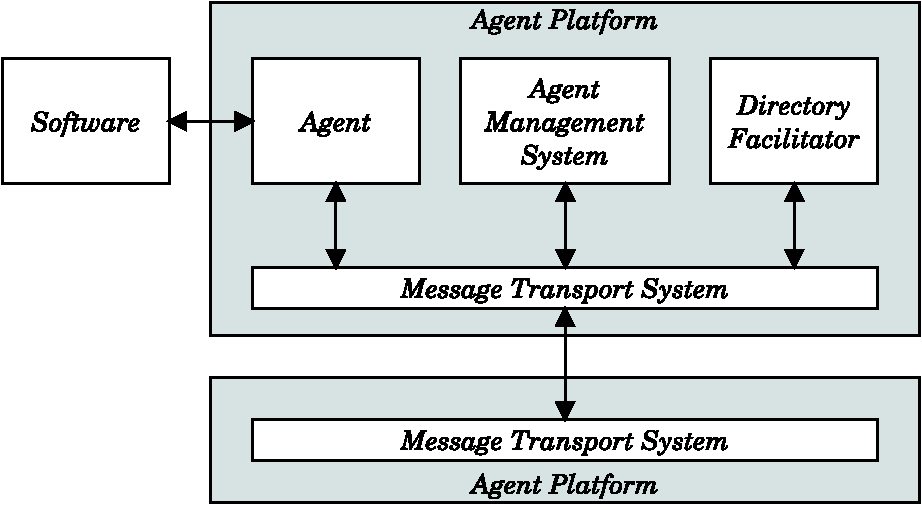
\includegraphics[width=2.5in]{figures/pdf/AMSdiagram.pdf}
%	\caption{
%		Agent Management Reference Model, as specified by FIPA and implemented by JADE. \apiname{} only supports a single Agent Platform.
%	}
%	\label{fig:AMSdiagram}
%\end{figure}

% DF 
The \gls{DF} is a component that provides a yellow page service and is part of the FIPA Agent Management Specification. It allows one agent to perform searches about agents rendering specific services. Only agents that are registered in the DF will be indexed and agents can register and deregister themselves at any time.

% DF Agent Description
When searching the DF, agents can use templates that filter the search results. A DF Agent Description represents this template and contains the fields listed in Table \ref{tab:dfAgentDescription}.

\begin{table}
	\normalsize
	\caption{Fields of the DF Agent Description used to filter results of the DF service.}
	\label{tab:dfAgentDescription}
	\begin{center}
		\begin{tabular}{c|c}
		\hline
		\textbf{Parameter} & \textbf{Description} \\
		\hline
		\texttt{name} & The identifier of the agent \\
		\hline
		\texttt{services} & A list of services supported by this agent \\
		\hline
		\texttt{protocol} & A list of interaction protocols supported by the agent. \\
		\hline
		\texttt{ontology} & A list of ontologies known by the agent. \\
		\hline
		\texttt{language} & A list of content languages known by the agent. \\
		\hline
		\end{tabular}
	\end{center}
\end{table} 

% MTS
The \gls{MTS} is a service for transportation of ACL messages between agents. It is responsible for resolving agent addresses, in order to be able to deliver those messages. The MTS may request information from the AMS to perform this address resolution.

% AMS
The AMS is a mandatory component in FIPA-compliant agent platforms. Its purpose is to manage the agent platform, namely the creating and deletion of agents.

% ACL Message
The ACL Message is the envelope that contains the details for communication. \gls{ACL} stipulates what fields a message should contain. Table \ref{tab:fipaACLMessage} was adapted from the FIPA ACL Message structure specification and contains the list of fields in a message. Not all of them are mandatory. FIPA specifies the \texttt{performative} as the only mandatory field, although the \texttt{sender}, \texttt{receiver} and \texttt{content} are expected to be present.

\begin{table}
	\normalsize
	\caption{FIPA ACL Message Parameters. The highlighted fields are the ones featured in the current version of \apiname{}.}
	\label{tab:fipaACLMessage}
	\begin{center}
		\fboxsep1pt
		\begin{tabular}{c|c}
		\hline
		\textbf{Parameter} & \textbf{Category of Parameters} \\
		\hline
		\colorbox{Apricot}{\texttt{performative}} & Type of communicative acts \\
		\hline
		\colorbox{Apricot}{\texttt{sender}} & \multirow{3}{*}{Participant in communication} \\
		\cline{1-1}
		\colorbox{Apricot}{\texttt{receiver}} \\
		\cline{1-1}
		\texttt{reply-to}  \\
		\hline
		\colorbox{Apricot}{\texttt{content}} & Content of message \\
		\hline
		\texttt{language} & \multirow{3}{*}{Description of Content} \\
		\cline{1-1}
		\texttt{encoding} \\
		\cline{1-1}
		\colorbox{Apricot}{\texttt{ontology}} \\
		\hline
		\colorbox{Apricot}{\texttt{protocol}} & \multirow{5}{*}{Control of conversation} \\
		\cline{1-1}
		\colorbox{Apricot}{\texttt{conversation-id}} \\
		\cline{1-1}
		\texttt{reply-with} \\
		\cline{1-1}
		\texttt{in-reply-to} \\
		\cline{1-1}
		\colorbox{Apricot}{\texttt{reply-by}} \\
		\hline
		\end{tabular}
	\end{center}
\end{table} 

% Protocols In FIPA
FIPA Interaction Protocols typify communication interactions among agents by specifying two roles: initiator (the agent starting the interaction) and responder (a participant in the interaction). Each protocol defines precisely which messages are sent by each role ad in which sequence.

% Behaviors in JADE
In JADE, every agent activity is programmed through the notion o behaviours. For interaction protocols, typically behaviour-pairs are used for each side of the interaction, and JADE's API supports the most important protocols with built-in initiator and responder behaviours.
% Implementing these protocols.
In order to create an application using these protocols, programmers only need to extend these behaviours and implement the message handlers.
All the complexity regarding the interaction and networking infrastructure is hidden and taken care of by JADE, allowing the programmer to focus on the implementation of agent behaviour.